\documentclass[final,hyperref={pdfpagelabels=false}]{beamer}
\usepackage{grffile}
\mode<presentation>{\usetheme{I6pd2}}
\usepackage[english]{babel}
\usepackage[latin1]{inputenc}
\usepackage{amsmath,amsthm, amssymb, latexsym}
\boldmath
\usepackage[orientation=landscape,size=a0,scale=1.4,debug]{beamerposter}
\usepackage{array,booktabs,tabularx}
\newcolumntype{Z}{>{\centering\arraybackslash}X}
\newcommand{\pphantom}{\textcolor{ta3aluminium}}
\usepackage{biblatex}

\listfiles
 
\title{\LARGE Big Data Analytics Pipeline for the Analysis of TESS Full Frame Images}
\author{Matthew Wampler-Doty \& Dr. John Doty}
\institute[Noqsi Aerospace]{Noqsi Aerospace, Ltd. \& MIT}
\date[]{}
\newlength{\columnheight}
\setlength{\columnheight}{105cm}

\begin{document}
\begin{frame}
  \begin{columns}
    \begin{column}{.49\textwidth}
      \begin{beamercolorbox}[center,wd=\textwidth]{postercolumn}
        \begin{minipage}[T]{.95\textwidth}  % tweaks the width, makes a new \textwidth
          \parbox[t][\columnheight]{\textwidth}{
            \begin{block}{Introduction}
            The goals of this research are two fold:
              \begin{itemize}
              \item Create a \emph{high fidelity} simulation of the TESS Full Frame Images (FFI)
              \item Develop data processing system that takes the TESS FFIs and looks for items such as:
              \begin{itemize}
              	\item Tidal disruption events
	        \item Gamma-ray burst afterglow
		\item Low surface brightness structures
		\item Unusual variable objects
		\item Exoplanets around non-targeted stars
              \end{itemize}
              \end{itemize}              
            \end{block}

            \vspace{2cm}
            \begin{block}{Conventional Data Processing Pipeline}
              
\includegraphics[width=0.95\linewidth]{figures/Conventional_Pipeline.pdf}
            \end{block}

            \vspace{2cm}
            \begin{block}{Our Data Processing Pipeline}
              
\includegraphics[width=0.95\linewidth]{figures/Our_Pipeline.pdf}
            \end{block}

          }
        \end{minipage}
      \end{beamercolorbox}
    \end{column}
    % ---------------------------------------------------------%
    % end the column

    % ---------------------------------------------------------%
    % Set up a column 
    \begin{column}{.49\textwidth}
      \begin{beamercolorbox}[center,wd=\textwidth]{postercolumn}
        \begin{minipage}[T]{.95\textwidth}
          \parbox[t][\columnheight]{\textwidth}{
            \begin{block}{Simulated TESS Full Frame Image}
            Image generated by Zach Berta-Thompson
              \begin{columns}
                \begin{column}{.60\textwidth}
                \begin{itemize}
                    \item Images generated in time series
                    \item Stars from the SDSS, Hubble, and OPTICAL catalogs are sampled to make simulate sky image
                    \begin{itemize}
                    	\item Catalogs of asteroids, comets, and other transients will also be employed
			\item Informs the \emph{Sky Model} used in the processing pipeline
                    \end{itemize}
                    \vfill
                    \item Optics, CCD detector physics, and electronics are simulated giving rise to a 2D binary image
                    \begin{itemize}
                    	\item Every photon from every star is independent, so this image can be rapidly generated using parallelization technologies like \texttt{CUDA} 
                    \end{itemize}
                    \vfill
                    \item Cosmic rays are also simulated, but removed using the \emph{central 8/10 method}
                    \vfill
                \end{itemize}
                \end{column}
                \begin{column}{.38\textwidth}
                  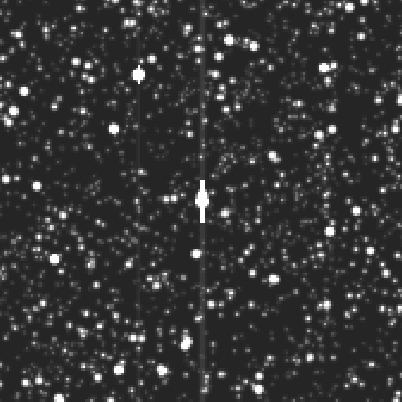
\includegraphics[width=0.80\linewidth]{figures/ffi_simulation.jpg}
		\end{column}
	       \end{columns}
            \end{block}
            \vspace{1cm}
            \begin{block}{Evaluation}
            	\begin{itemize}
			\item Series of images give rise to time series which can be mined looking for various objects and events
			\item To evaluate the performance of a particular mining algorithm, downlink data is simulated 
			\item Comparison of algorithms uses various statistical performance measurements:
				\begin{columns}
                			\begin{column}{.60\textwidth}
			        $$ F_1 = \frac{A}{A + \frac{B + C}{2}} $$
			       
			       $$ Markedness = \frac{A}{A + B} + \frac{C}{C+D}$$
			       
			       $$ Informedness = \frac{A}{A+C} + \frac{B}{B+D}$$
			       \end{column}
                		       \begin{column}{.38\textwidth}
		                         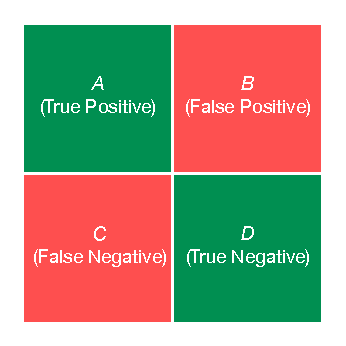
\includegraphics[width=0.65\linewidth]{figures/truth_table}
	       		       \end{column}
			       \end{columns}
			       \begin{center}
			       	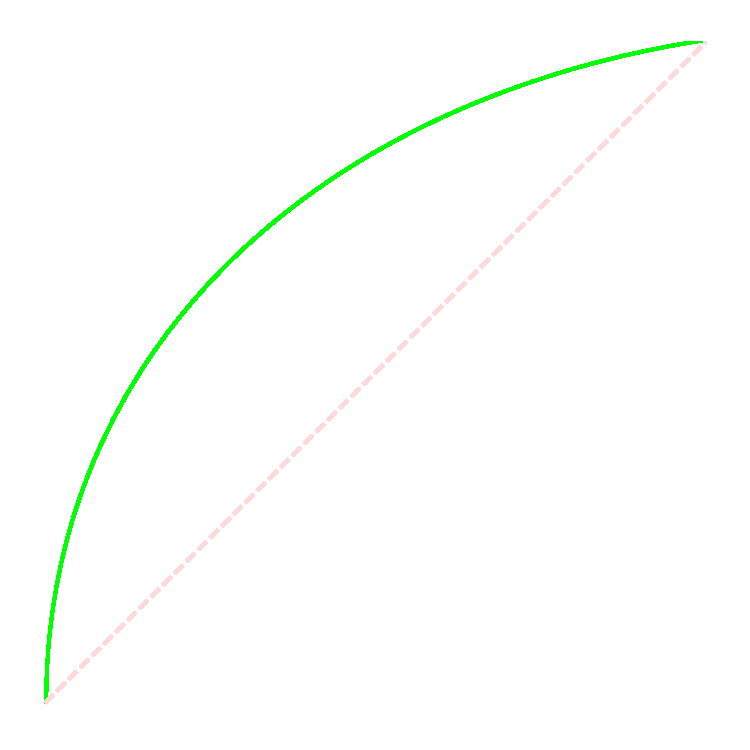
\includegraphics[width=0.30\linewidth]{figures/ROC}
			       \end{center}
                \end{itemize}
            \end{block}
          }

        \end{minipage}
      \end{beamercolorbox}
    \end{column}
    % ---------------------------------------------------------%
    % end the column
  \end{columns}
  \vskip1ex
  %\tiny\hfill\textcolor{ta2gray}{Created with \LaTeX \texttt{beamerposter}  \url{http://www-i6.informatik.rwth-aachen.de/~dreuw/latexbeamerposter.php}}
  \tiny\hfill{Created with \LaTeX \texttt{beamerposter}  \url{http://www-i6.informatik.rwth-aachen.de/~dreuw/latexbeamerposter.php} \hskip1em}
\end{frame}
\end{document}


%%%%%%%%%%%%%%%%%%%%%%%%%%%%%%%%%%%%%%%%%%%%%%%%%%%%%%%%%%%%%%%%%%%%%%%%%%%%%%%%%%%%%%%%%%%%%%%%%%%%
%%% Local Variables: 
%%% mode: latex
%%% TeX-PDF-mode: t
%%% End:
